%\usepackage[normalem]{ulem}
%\useunder{\uline}{\ul}{}

\section{Results}

%This section should include the following:
%
%\begin{itemize}
%
%	
%	\item Details and explanations of results obtained (which itself could have
%		sub-sections). This is where you should provide tables, graphs, and/or
%		figures that illustrate your results. If you have created a new
%		application, include screenshots of it in action. You should also provide a
%		link to your application if it is web-based.
%
%\end{itemize}
%
%You should entitle these sections and sub-sections with names that describe the
%key points (for example, instead of ``methods we use", the heading
%``Statistical-Based Learning" would be more informative). The Methods and
%Results sections should together be approximately 3-4 pages in length.

We produced a highly accessible CAD program suitable for use laser cutting. The accessibility of 2to3D can be attributed to the fact that the program runs entirely in the browser (thus requiring no additional software beyond a modern browser), and that is strips away all non-essential drawing features. Currently 2to3D only supports the creation of drawings intended for translation into cutting paths. Figure XX depicts a full digital fabrication workflow using 2to3D. The figure depicts the design of a press-fit box using 2to3D. The laser cutter available for use utilized CorelDRAW for CAM so the drawing was exported from 2to3D as a SVG and imported to CorelDRAW. 

\begin{figure}[H]
  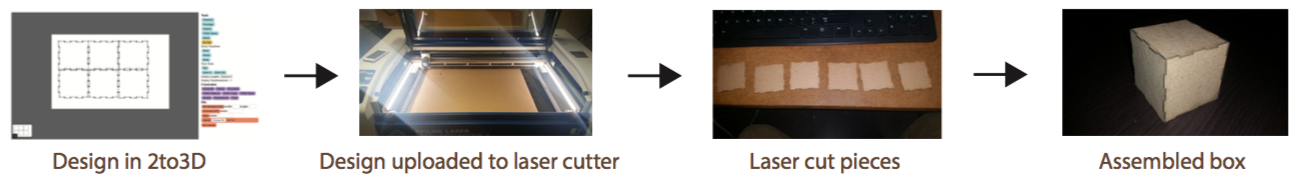
\includegraphics[width=\linewidth]{usingProgram.jpg}
  \caption{Full digital fabrication workflow using 2to3D. The laser cutter we had access to used CorelDraw for CAM so the drawing was created in 2to3D and imported to CorelDraw just for printing.}
  \label{fig:usingProgram}
\end{figure}

2to3D has a simple design that displays all tools to the user without being overwhelm and which also immediately and constantly conveys program state by highlighting the current tool and changing the cursor style. Figures X and X are screenshots of the program.

\begin{figure}[H]
  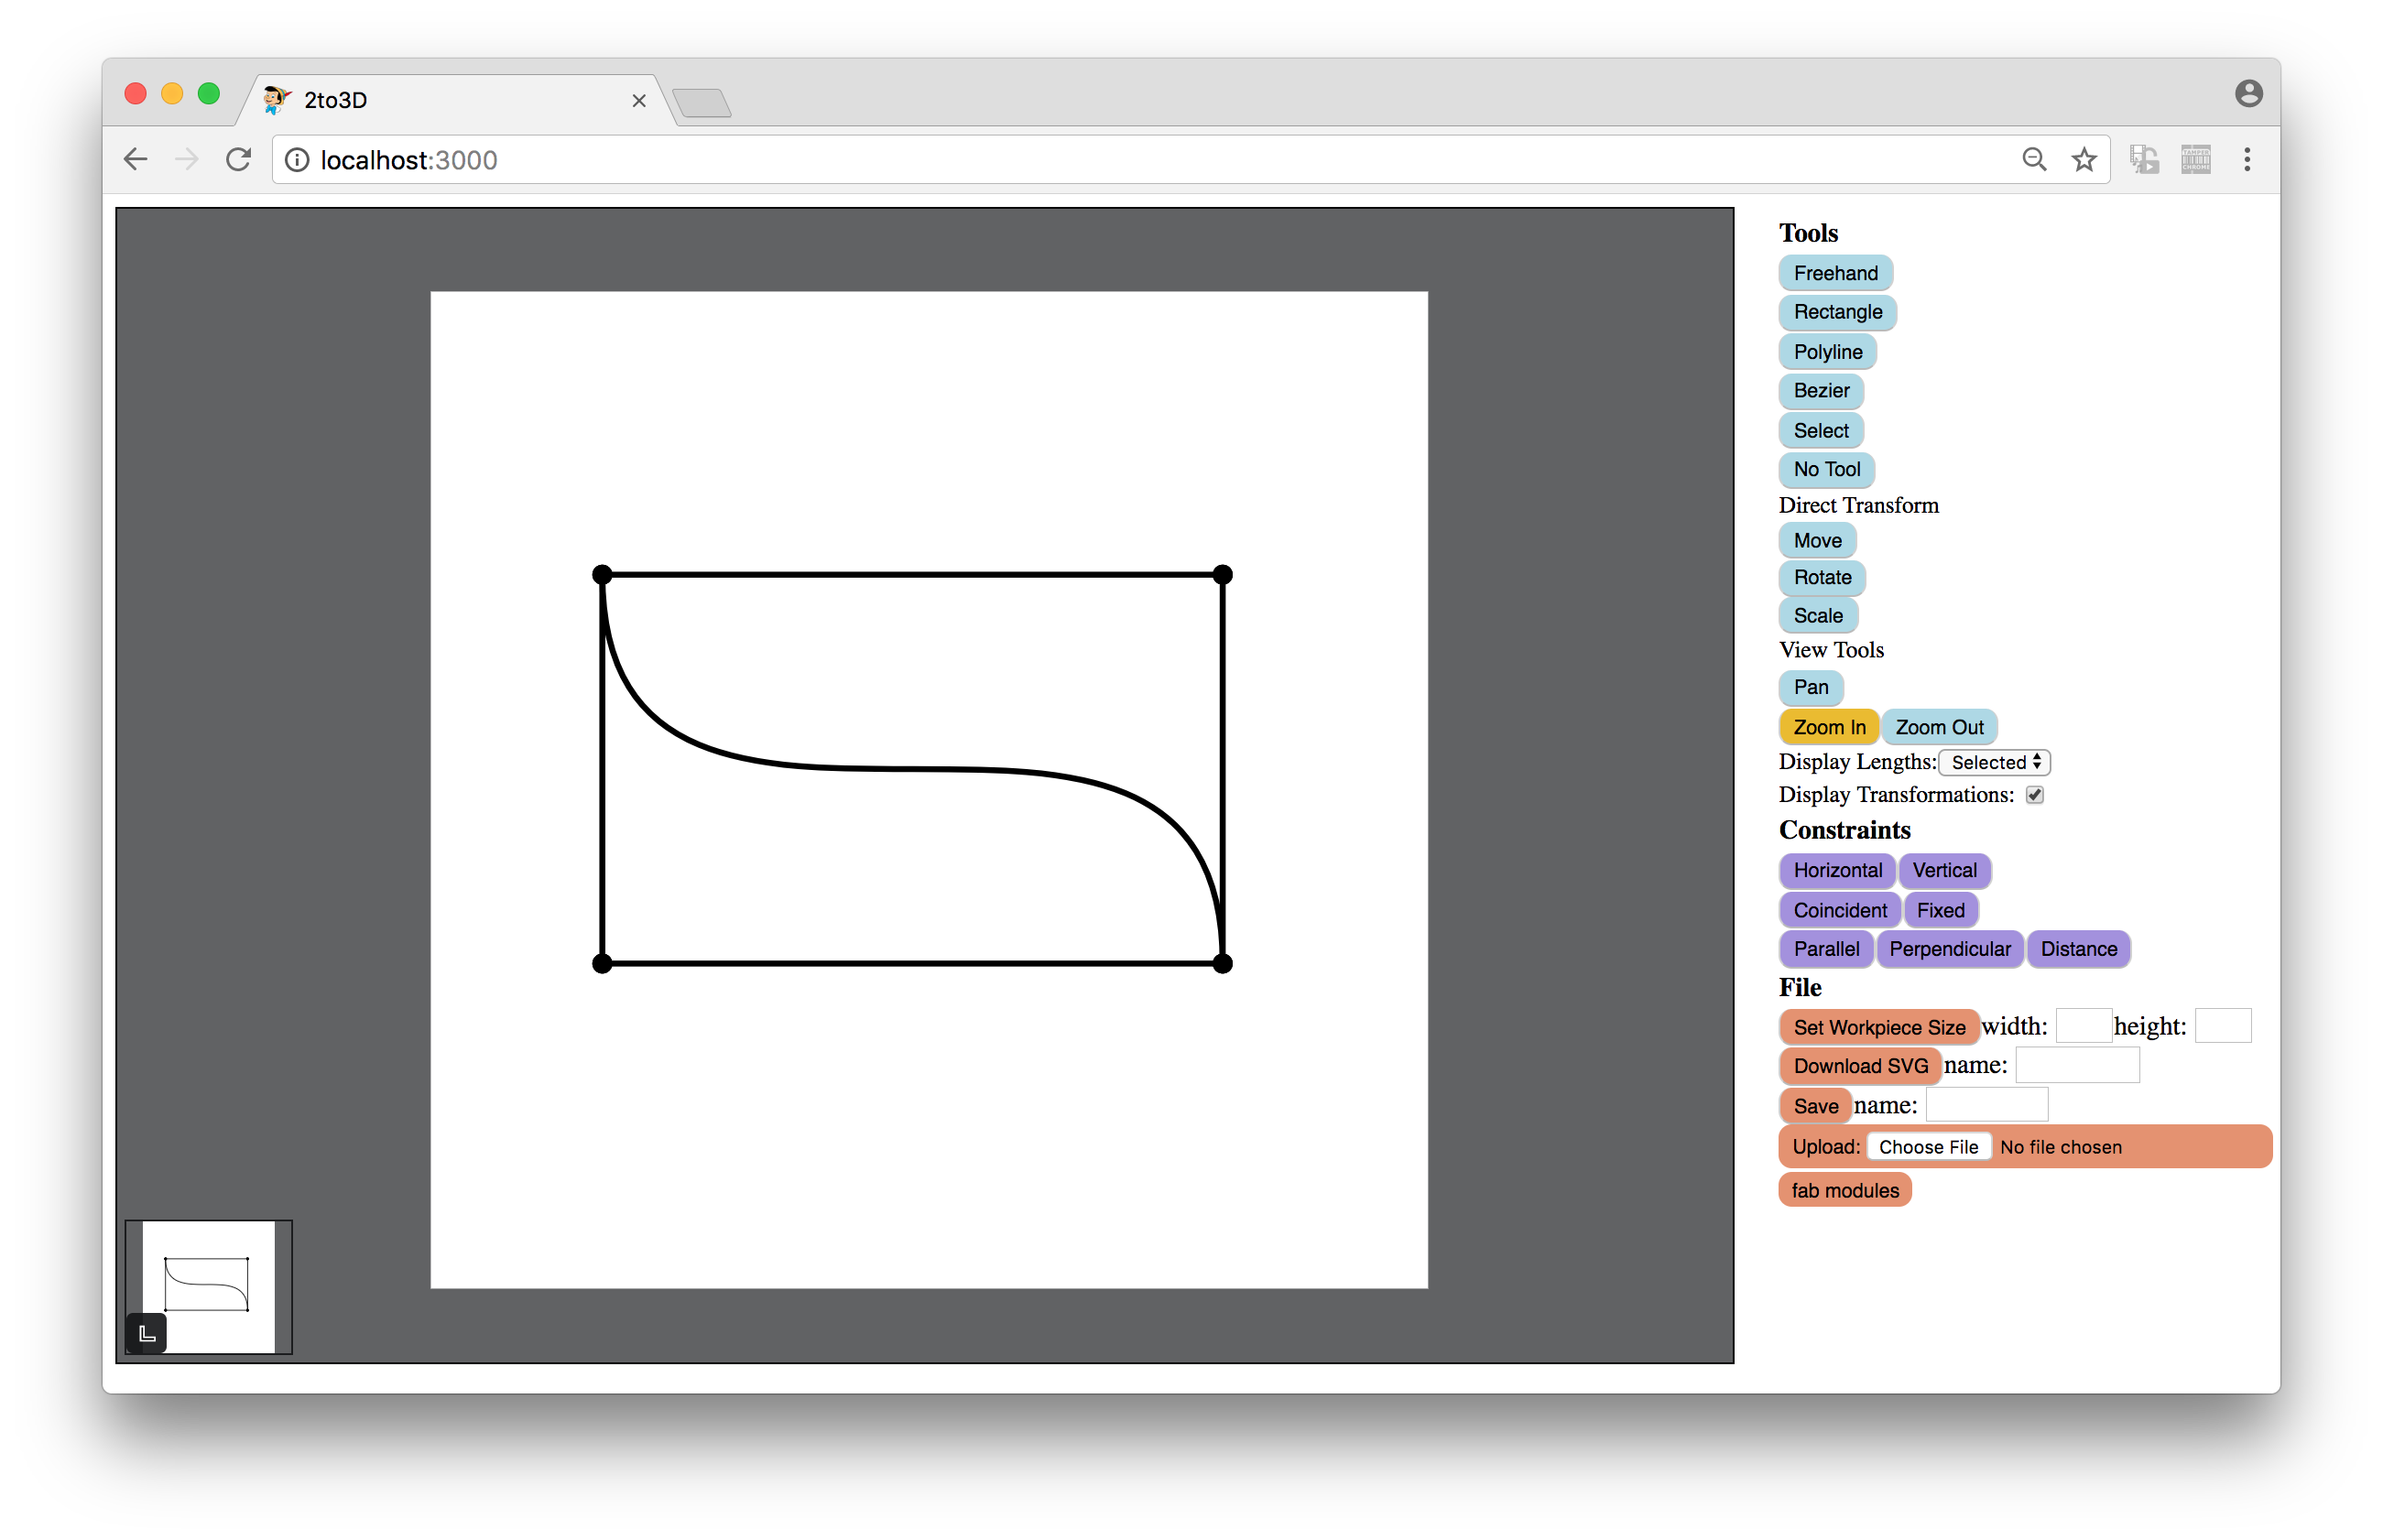
\includegraphics[width=\linewidth]{screenshot.png}
  \caption{}
  \label{fig:screenshot}
\end{figure}

\begin{figure}[H]
  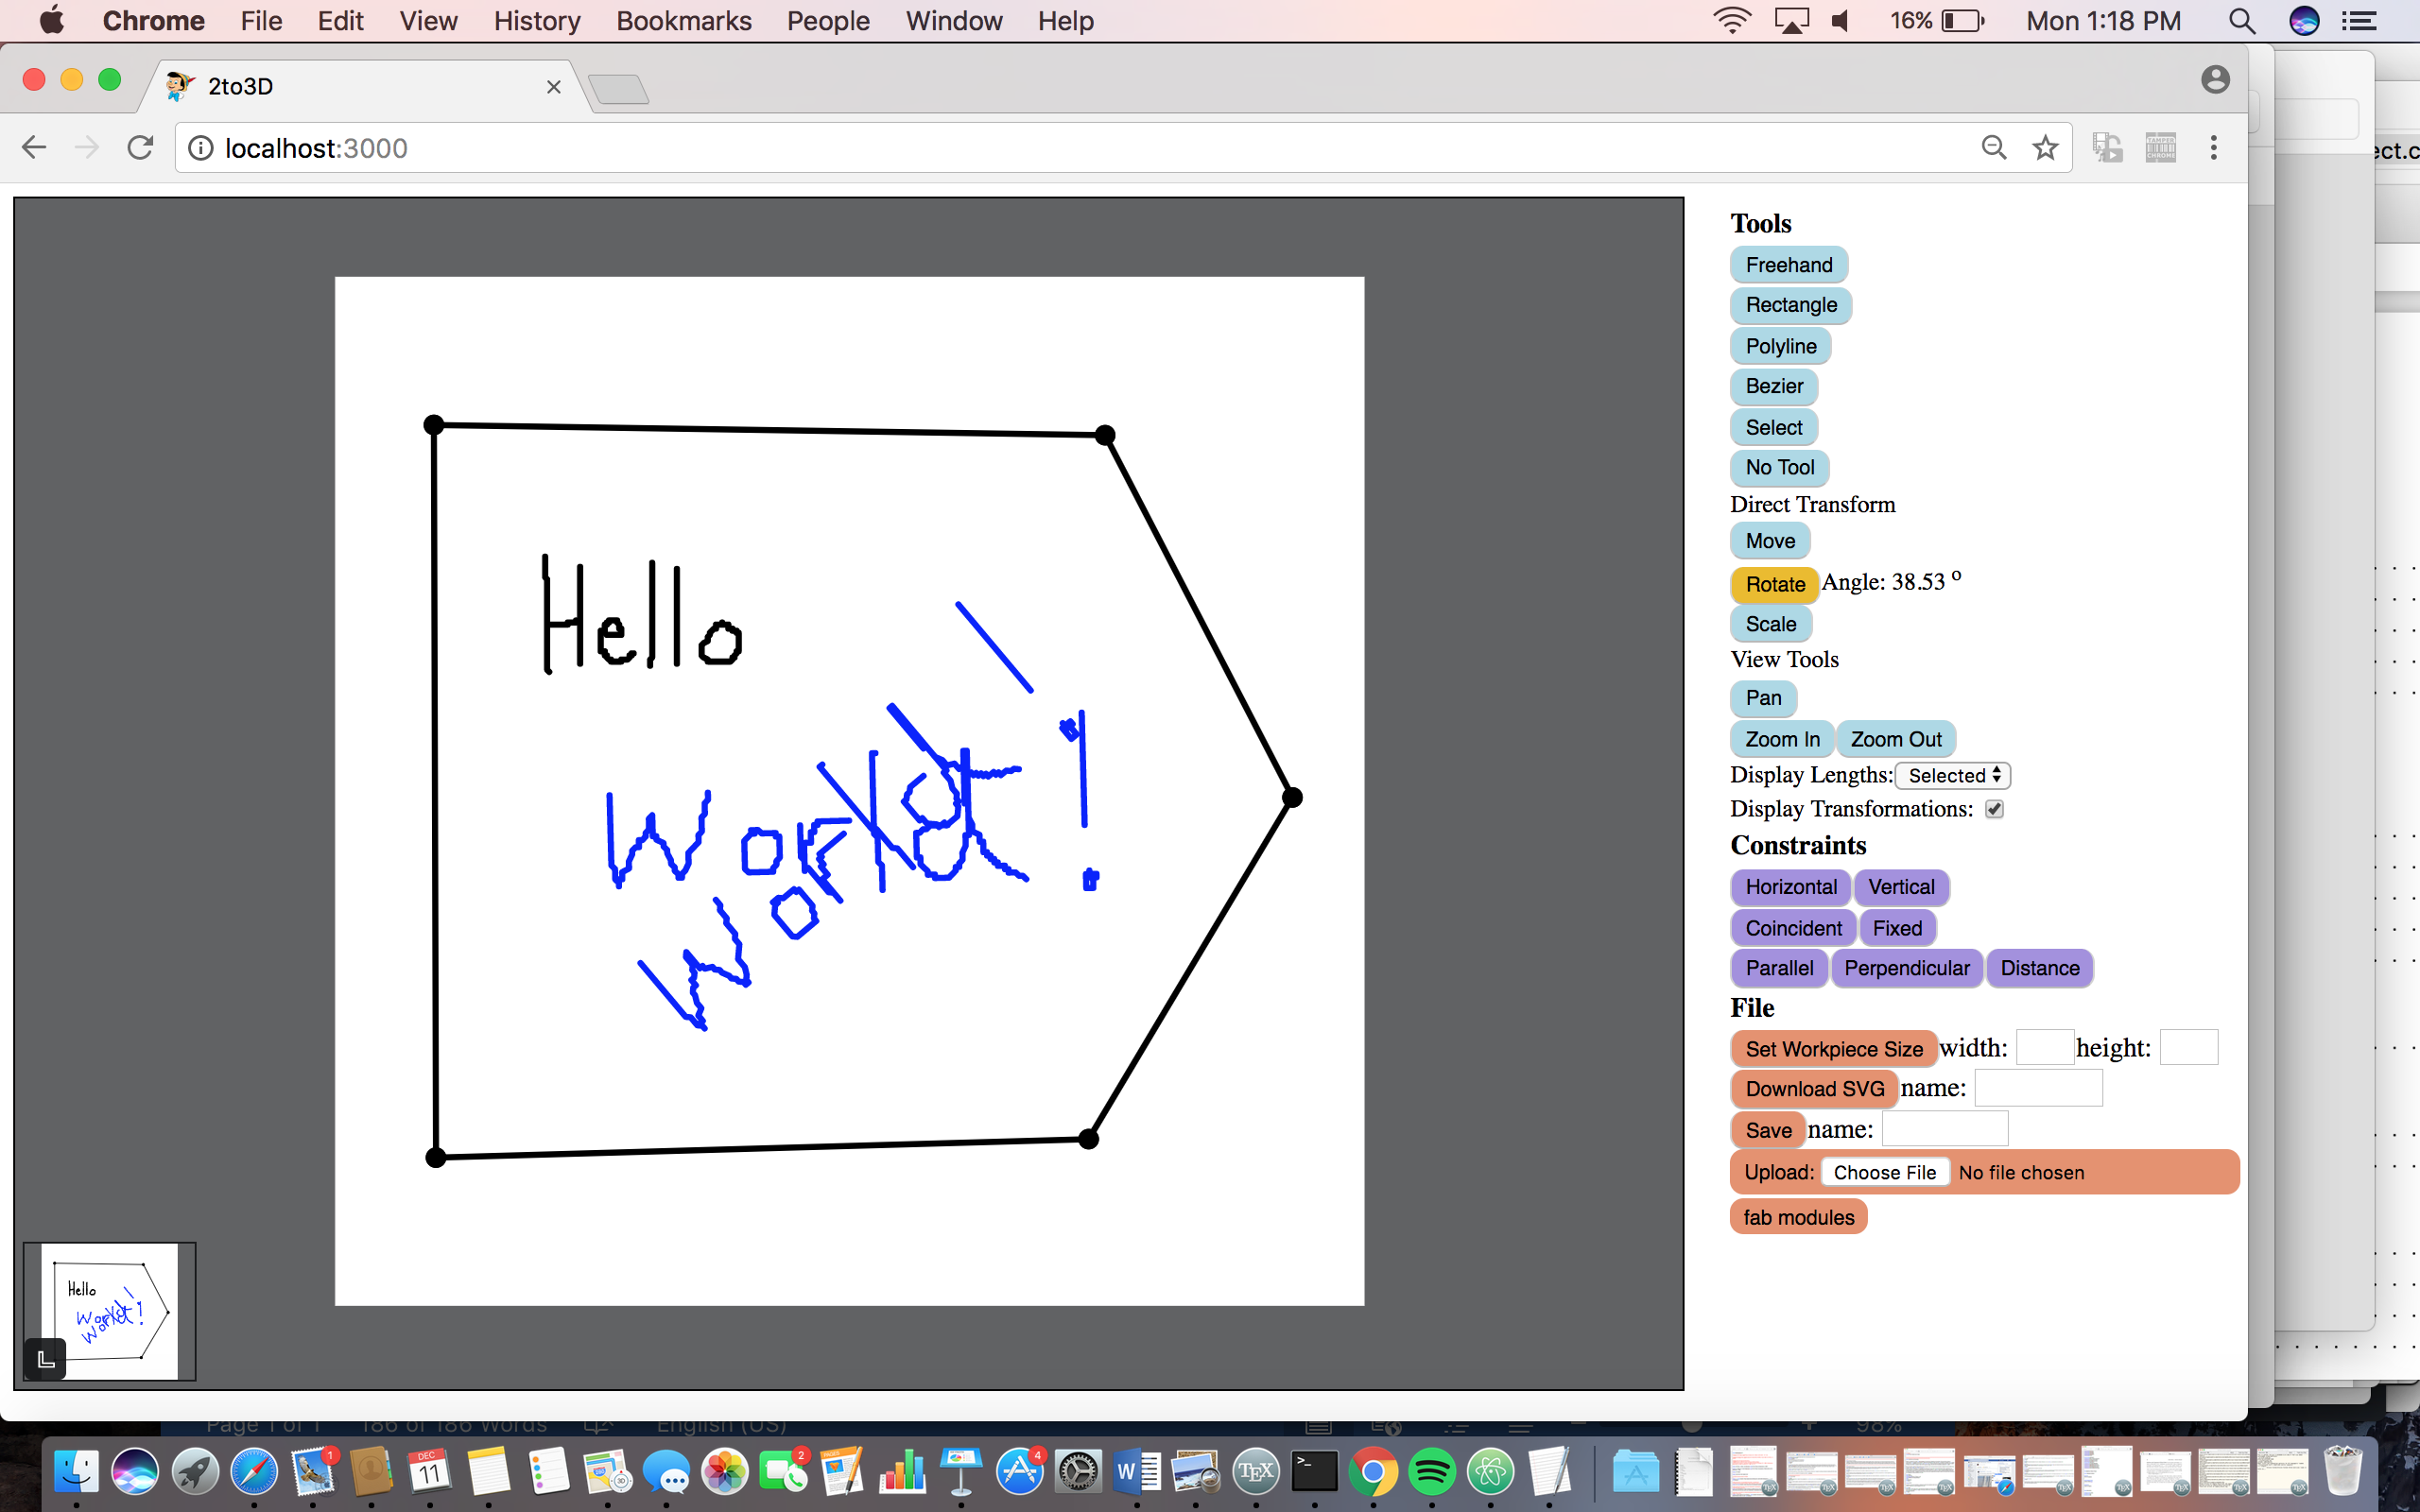
\includegraphics[width=\linewidth]{screenshot2.png}
  \caption{}
  \label{fig:screenshot2}
\end{figure}

In addition to the shapes and constraints discussed above 2to3D also supports a myriad of other features. This includes direct transformations - rotations, moves, and scales - that break constraints of transformed objects. This allows the user to make direct edits to drawing geometry that will exactly reflect user's intention. The drawing area supports zooming in/out and panning and the workpiece size is adjustable which facilitates creation of designs on any scale. SVG exports draw dimensions from workpiece size which simplifies the CAM process if the user decides to match drawing dimensions to laser cutter bed size. Hotkeys support swift and smooth workflows and copy and paste capabilities allow users to quickly create redundant geometry. A save and upload feature also allows users to continue work on unfinished projects or share designs with others. A full list of features can be found in Table XX.

\begin{table}[H]
\centering
\caption{Capabilities of 2to3D.}
\label{my-label}
\begin{tabular}{|l|l|l|l|}
\hline
\multicolumn{2}{|l|}{{\ul \textbf{Drawing}}}                                                                                                                                                        & \multicolumn{2}{l|}{{\ul \textbf{Navigation}}}                                                                                                                                               \\
\multicolumn{2}{|l|}{\begin{tabular}[c]{@{}l@{}}Freehand\\ Rectangle\\ Polyline\\ Bezier\end{tabular}}                                                                                              & \multicolumn{2}{l|}{\begin{tabular}[c]{@{}l@{}}Pan\\ Zoom in/out\end{tabular}}                                                                                                               \\ \hline
\multicolumn{2}{|l|}{{\ul \textbf{Direct Transformations}}}                                                                                                                                         & \multicolumn{2}{l|}{{\ul \textbf{Display Options}}}                                                                                                                                          \\
\multicolumn{2}{|l|}{\begin{tabular}[c]{@{}l@{}}Move\\ Rotate\\ Scale\end{tabular}}                                                                                                                 & \multicolumn{2}{l|}{\begin{tabular}[c]{@{}l@{}}Lengths\\ Transformation values\end{tabular}}                                                                                                 \\ \hline
\multicolumn{2}{|l|}{{\ul \textbf{Constraints}}}                                                                                                                                                    & \multicolumn{2}{l|}{{\ul \textbf{Other}}}                                                                                                                                                    \\
\multicolumn{2}{|l|}{\begin{tabular}[c]{@{}l@{}}Horizontal (line)\\ Vertical (line)\\ Coincident (points)\\ Fixed (points)\\ Parallel (lines)\\ Perpendicular (lines)\\ Length (line)\end{tabular}} & \multicolumn{2}{l|}{\begin{tabular}[c]{@{}l@{}}Click and drag points\\ Download SVG\\ Save drawing\\ Upload drawing\\ Copy/Paste\\ Delete\\ Hotkeys\\ Workpiece size adjustable\end{tabular}} \\ \hline
\end{tabular}
\end{table}